\documentclass[a4paper,11pt]{jarticle}
\usepackage{ics-thesis}
\usepackage{amssymb}
\usepackage[dvipdfmx]{graphicx}
\usepackage{subcaption}
\pagestyle{bachelorthesis}    % 卒論・規定の.styファイルを使う場合
%
\title{サイボーグインセクトによる迅速な被災者発見のための自己組織型移動制御手法の提案}
\author{北浦 直}
\supervisor{若宮 直紀 教授}
\deadline{2019年2月12日}
%
\begin{document}
	\titlepage    % 規定の.styファイルを使う場合
	\abstract     % 規定の.styファイルを使う場合
	%%%%%%%%%%%%%%%%%%%%%
	% 内容梗概本文
	%%%%%%%%%%%%%%%%%%%%%
	\keyword
	%%%%%%%%%%%%%%%%%%%%%
	% キーワード
	%%%%%%%%%%%%%%%%%%%%%
	\tableofcontents    % 目次
	%
	%%%%%%%%%%%%%%%%%%%%%
	% 本文
	%%%%%%%%%%%%%%%%%%%%%
	%
	\section{はじめに}
	災害が起きた場合,倒壊した建物内に被災者が取り残されることが起こりうる.
	倒壊した建物内に捕らわれた被災者の探索において,現在は災害救助犬やスコープカメラなどの人間の能力を補助するような手法が広く使われている.
	しかし,倒壊した建物内は人間や災害救助犬が入れないような環境であることが多い.%ここで例とかあったほうがいいかも
	また,救助活動の中で2次災害が起きてしまう事例も少なくない.
	そこで,現在の探索手法では探索できないような狭い空間を探索可能で,探索中の2次災害の危険性を低くすることができるサイボーグインセクトを用いた被災者探索の研究がなされている.

	サイボーグインセクトを被災者探索に活用するための研究としてCINEMa(Cyborg Insect Networks for Exploration and Mapping)があげられる.
	この研究の中では,サイボーグインセクトへ制御を与えて任意の方向へ向かわせたり,サイボーグインセクトが位置推定をするためのアルゴリズムの実験がされていたりする.
	しかし,CINEMaはがれきなどが散乱するような悪条件下における被災者探索のための構成要素の確立は行われているが,それらを用いて被災者探索を効率的に行うためのアルゴリズムなどは提案されていない.
	つまり,群で探索しているにも拘らず複数個体がほぼ同一の場所を探索することで空間全体を探索するのにかかる時間が増加してしまう恐れがある.
		
	また,自律的なレスキューロボットが行う自律的なアルゴリズムの1つであるフロッキングという手法がある.
	フロッキングとは,周囲のロボットに対して,Separation,Alignment,Chesionの3つの動作をとることで複数個体が群れとなって動くようなアルゴリズムである.
	このフロッキングを被災者探索に適用される研究が行われているが,フロッキングをサイボーグインセクトに適用して被災者探索を実現している研究はなされていない.
	また,これらの研究でなされているフロッキングは基本的に連続で操作を行っており,断続的に制御を行っている研究は少ない.
	しかし,サイボーグインセクトに与えるフロッキングの制御は生物に電気信号を流すためできるだけ頻度が低いことが望ましい.
	
	そこで,本研究ではCINEMaで提案されているようなサイボーグインセクトの群れに対するフロッキング制御手法の提案を行う.ここでは,サイボーグインセクトに対する断続的なフロッキング制御でも探索にかかる時間の短縮ができることを確認する.
	
	以降,第章では,
	\section{サイボーグインセクト}
	この章では,本研究で考えるサイボーグインセクトの概要と,サイボーグインセクトに取り付けられる機材,サイボーグインセクトに関する条件の説明を行う.
	\section{フロッキング}
	この章では,フロッキングについて説明する.
	\section{サイボーグインセクトのモデル}
	\label{sec:algorithm}
	この章では,サイボーグインセクトが制御を受けていない場合の動きのモデルについて説明を行う.
	\begin{figure}
		\centering
		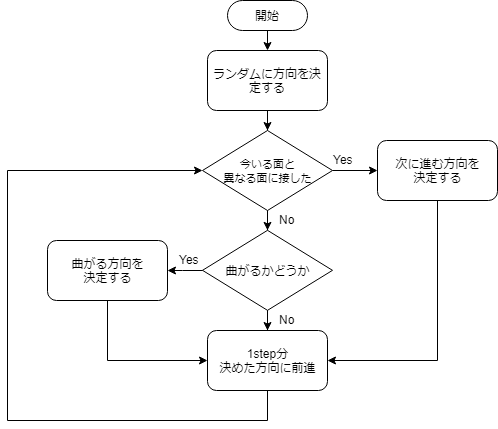
\includegraphics[width=0.5\linewidth]{png/Untitled.png}
		\caption[アルゴリズムのフローチャート]{制御されていないサイボーグインセクトのアルゴリズムのフローチャート}
		\label{fig:algorithm}
	\end{figure}
	
	制御をされていないサイボーグインセクトは,図\ref{fig:algorithm}のフローチャートに示されているアルゴリズムに従って行動する.
	このアルゴリズムでの1stepは0.1秒とする.
	また,サイボーグインセクトの速度は 60cm/s とする\cite{speed}.
	
	\subsection{進行方向ベクトルの初期値決定}
	\label{random}
	探索が開始されたときに実行される.
	どの方向に進むのかをランダムに決定する.
	以下の章ではサイボーグインセクトが進む方向の単位ベクトルを進行方向ベクトルと呼ぶ.
		
	\subsection{進行方向ベクトルを変更するかの判定}
	\label{carb}
	サイボーグインセクトは,1step毎に現在の進行方向ベクトルを別の進行方向ベクトルに変更するかの判定を行う.
	この時に,進行方向ベクトルを変更する確率は1\%とする.
	
	\subsection{回転角の決定}
	現在の進行方向ベクトルからどれだけ回転するかの決定を行う.
	この時,現在の進行方向ベクトルから角度が大きく異なる進行方向ベクトルほど選択する確率が低くなるように設定した.
	また,現在接している面から別の面へ移動するようなベクトルには回転しないものとする.
	図\ref{fig:bend}のように赤い矢印であらわされるベクトルには回転する可能性が存在し,青のベクトルのように接する面が変わるベクトルには回転しないものとする.
	\begin{figure}
		\centering
		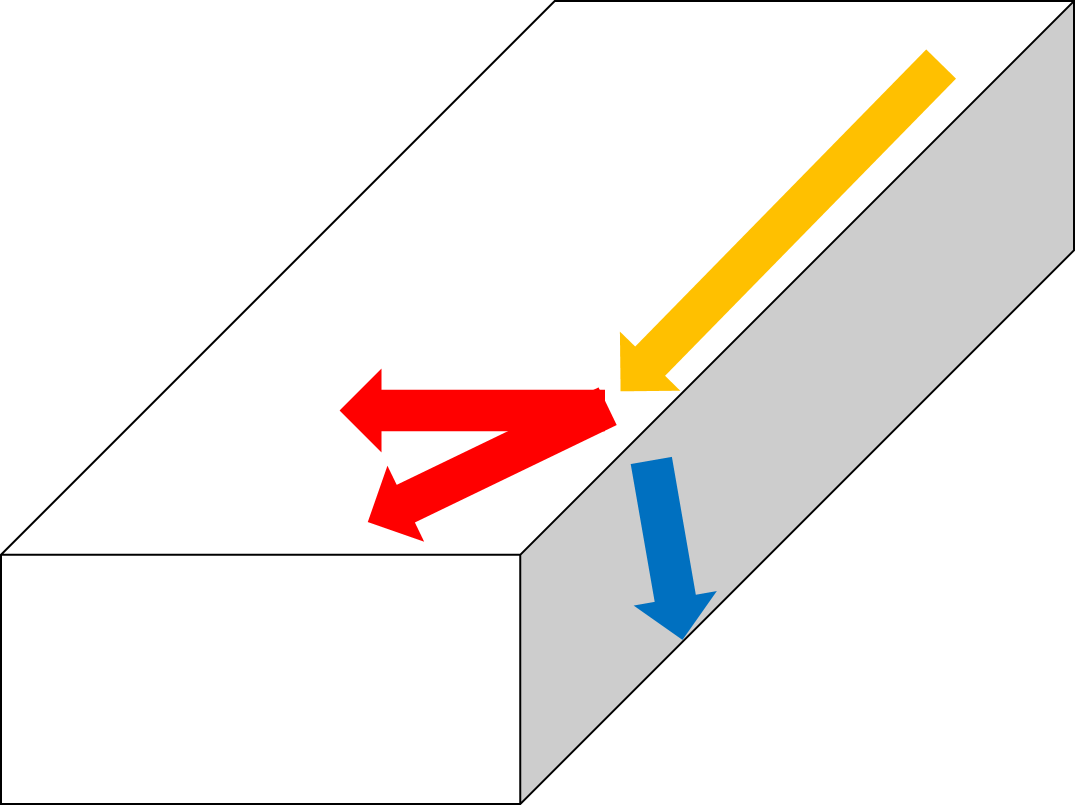
\includegraphics[width=0.35\linewidth]{png/bend.png}
		\caption[ベクトルの決定]{回転できるベクトル(赤)と回転できないベクトル(青)の例}
		\label{fig:bend}
	\end{figure}
	
	ここで,回転する角度は,平均0,分散$\frac{\pi}{6}$の正規分布に従って決定される.
	
	\subsection{1step分前進}
	サイボーグインセクトは,進行方向のベクトルに1step分前進する.
	また,途中で障害物があったり接している面が途切れたりなどで1step分の距離を進めない場合は,進めるところまで進み,その位置で停止する.
	
	\subsection{面と面が構成する境界線に接したかの判定}
	サイボーグインセクトは,現在いる場所が面と面が構成する境界線に接しているかどうかを1step毎に判定を行う.
	
	\subsection{次の進行方向ベクトルの決定}
	\label{vector}
	サイボーグインセクトは次の進行方向ベクトルを計算する.次に進行方向ベクトルの候補として,図\ref{fig:vec_surface}のような3種類のベクトルを計算する.この時,サイボーグインセクトがすでに境界線に沿って進んでいる場合は,図\ref{fig:vec_boader}のように,新しく接した境界線に沿うような2つのベクトルを計算する.
	\begin{enumerate}
		\item 境界線に平行なベクトル
		\item 境界線に平行な1.の逆ベクトル
		\item 現在の方向を保ちつつ,新しく接した面に平行なベクトル
	\end{enumerate}
	\begin{figure}
		\begin{minipage}{0.5\linewidth}
			\centering
			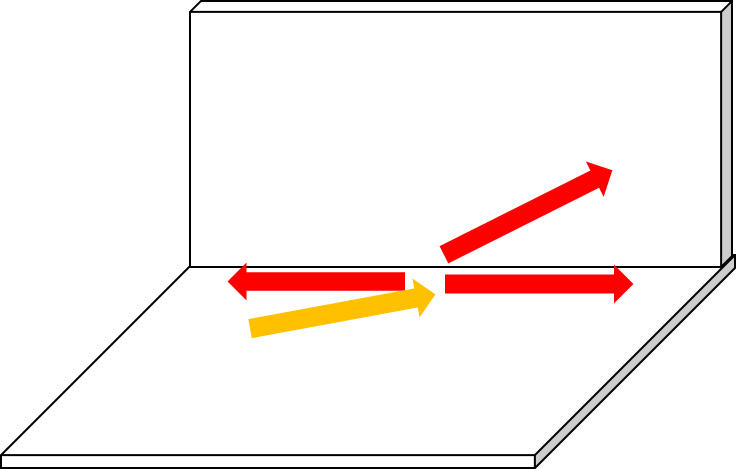
\includegraphics[width=1\linewidth]{png/vector.png}
			\subcaption{面上を進んでいる場合}\label{fig:vec_surface}
		\end{minipage}
		\begin{minipage}{0.5\linewidth}
			\centering
			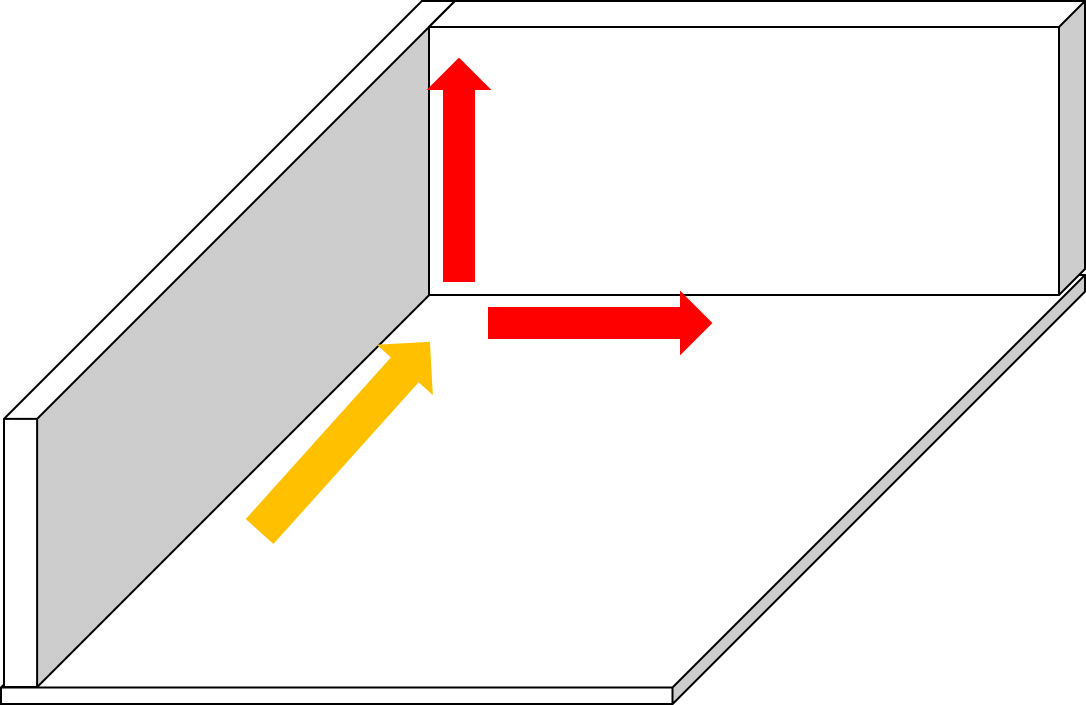
\includegraphics[width=1\linewidth]{png/vector2.png}
			\subcaption{境界線上を進んでいる場合}\label{fig:vec_boader}
		\end{minipage}\\
		\caption{次に進む方向のベクトル}
		\label{fig:vector}
	\end{figure}
	
	それぞれの具体的な計算方法は以下の章で説明する.
	\subsubsection{境界線に平行なベクトル}
	\label{boader}
	新たに接した境界線からベクトルを求めて,そのベクトルに平行な単位ベクトルを次の進行方向ベクトルの候補とする.
	\ref{fig:vec_boader}のように境界線上を進んでいる場合,新たに接した境界線が2つあるため,その2つを次の進行方向ベクトルの候補とする.
	
	\subsubsection{境界線に平行なベクトルの逆ベクトル}
	\ref{boader}章で求めたベクトルの逆ベクトルを次の進行方向ベクトルの候補とする.
	
	\subsubsection{現在の方向を保ちつつ,新しく接した面に平行なベクトル}
	\label{rotation}
	現在の進行方向ベクトルを新たに接した境界線を軸にして回転することで次の進行方向ベクトルの候補を計算する.
	現在の進行方向ベクトルの境界線に垂直な成分から,新しく検知した面に平行で境界線に垂直なベクトルに反時計回りでなす角を$ \phi $としたときに,現在の進行方向ベクトル$\vec{v}$を$\phi$だけ回転することで,次の進行方向ベクトルの候補$\vec{l}$が得られる.
	$\phi$の求め方は図\ref{fig:rotation}のようになる.
	
	\begin{figure}
		
		\begin{minipage}{0.5\linewidth}
			\centering
			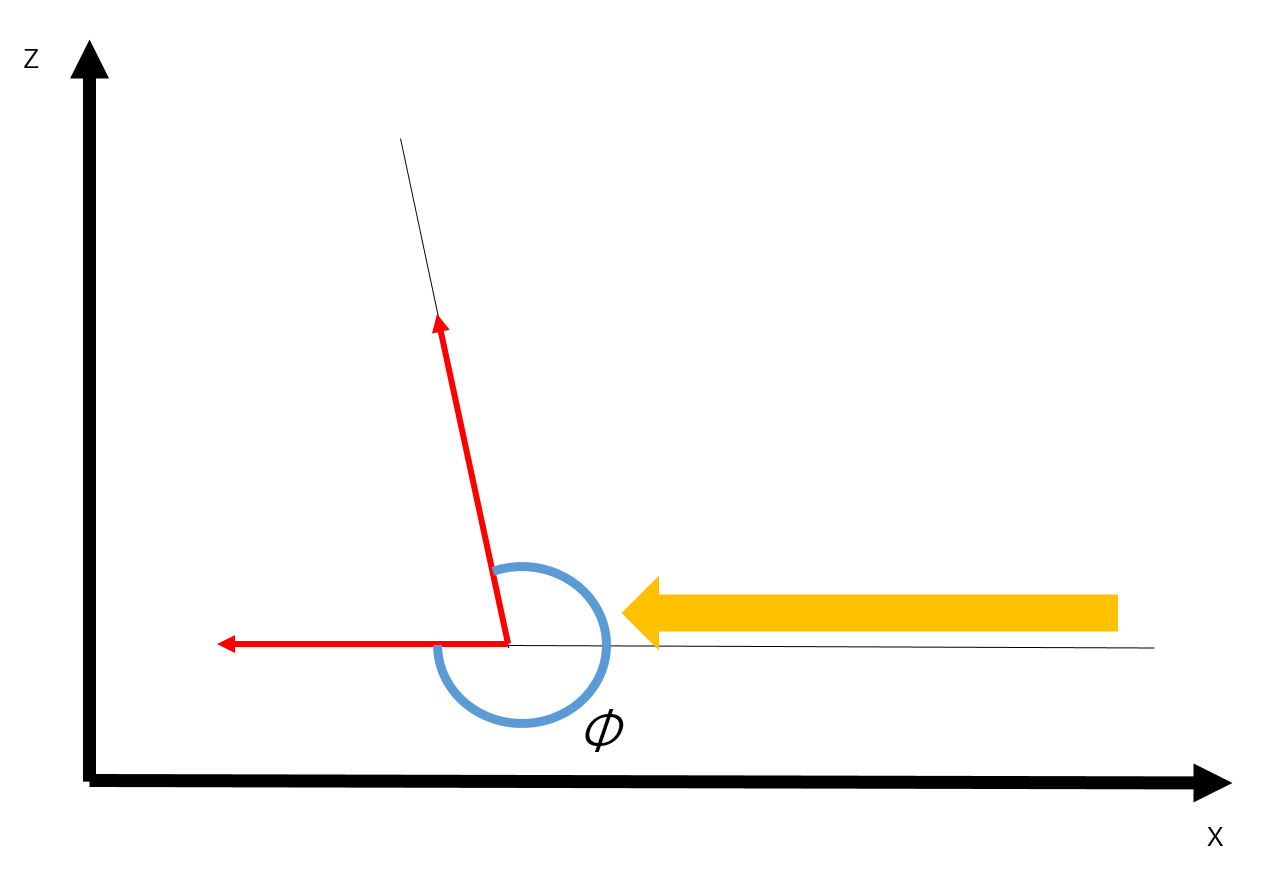
\includegraphics[width=1\linewidth]{png/rotation.png}
		\end{minipage}
		\begin{minipage}{0.5\linewidth}
			\centering
			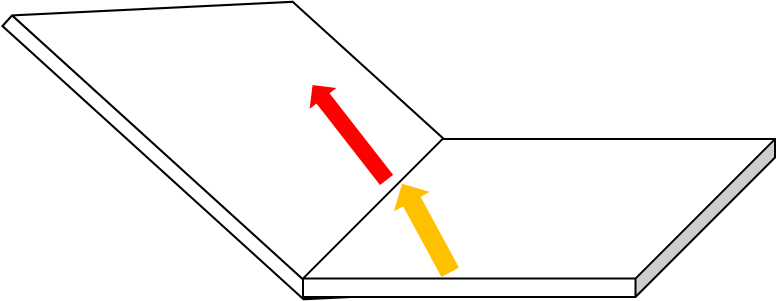
\includegraphics[width=1\linewidth]{png/sub.png}
		\end{minipage}
		\caption{なす角$\phi$の位置}
		\label{fig:rotation}
	\end{figure}
	
	境界線に平行なベクトルを$\vec{b} $とした際に,次の進行方向ベクトルの候補$\vec{l}$は式\ref{formula:l}によってあらわされる.
	\begin{equation}
	\label{formula:l}
	\vec{l} = R_{\vec{b}}(\phi)\vec{v}
	\end{equation}
	
	ここで$R_{\vec{b}}(\phi)$は境界線に平行なベクトル$\vec{b}$を軸に角度$\phi$だけ回転させる回転行列とする.
	回転行列$R_{\vec{b}}(\phi)$は式\ref{formula:rotation}で計算される.
	
	\begin{equation}
	\label{formula:rotation}
	R_{\vec{b}}(\phi)=\left( \begin{array}{ccc}
	b_x^2(1-\cos\phi)+\cos\phi & b_x b_y (1-\cos\phi) - b_z\sin\phi & b_z b_x (1-\cos\phi) + b_y\sin\phi \\
	b_x b_y (1-\cos\phi)+b_z \sin\phi & b_y^2 (1-\cos\phi) + \cos\phi & b_y b_z (1-\cos\phi) - b_x\sin\phi \\
	b_z b_x (1-\cos\phi)- b_y\sin\phi & b_y b_z (1-\cos\phi) + b_x \sin\phi & b_z^2 (1-\cos\phi) + \cos\phi \\
	\end{array} \right)
	\end{equation}
	
	\subsubsection{ベクトルの決定}
	\ref{boader}章から\ref{rotation}章で計算したベクトル$\vec{l}_i$から,次の進行方向ベクトルを決定する.
	次の進行方向ベクトルは,基準ベクトルとの差異による確率に従って決定される.
	基準ベクトルは,現在の進行方向ベクトルと重力ベクトルとの和によって計算される.
	まず,現在の方向ベクトル$ \vec{v} $と重力ベクトル$ \vec{g} $から基準となるベクトル$ \vec{a} $を計算する式は以下の通りである.
	\begin{equation}
	\vec{a} = \vec{v} +\frac{49}{60} \vec{g} 
	\end{equation}
	ここで,$ \vec{g} $の係数は,0.1秒分の自由落下の計算から求めている.
	
	次に,各ベクトルを選択する確率は式\ref{formula:prob}によって計算される.
	\begin{equation}
	\label{formula:prob}
	P(\vec{l}_i) = \frac{1}{n-1}(1 - \frac{|\vec{a} - \vec{x}_i |}{\sum_{k=1}^{n}|\vec{a} - \vec{x}_k|})
	\end{equation}
	
	ここで,$ \vec{l}_i $は\ref{boader}章から\ref{rotation}章で計算した次の進行方向ベクトルの候補で,$ i = (1,..,n) $である.
	
	\section{制御モデル}
	\label{sec:control}
	この章では,\ref{sec:algorithm}章で説明したサイボーグインセクトのモデルへの制御を説明する.
	
	この制御の目的は,空間全体の探索にかかる時間を短縮することである.
	また,サイボーグインセクトへの負担や消費電力の軽減のため,サイボーグインセクトに対して常に制御を行うのではなくある周期ごとに断続な制御を与える.
	
	制御を加える場合の全体のアルゴリズムは図\ref{fig:control}のフローチャートであらわされる.
	
	\begin{figure}
		\centering
		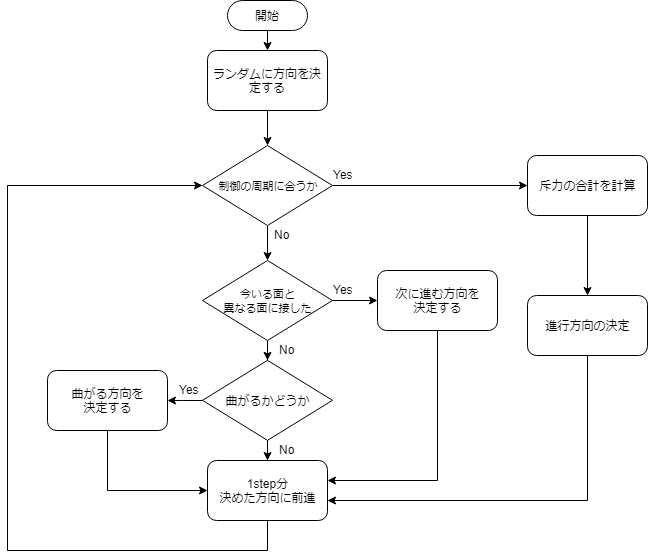
\includegraphics[width=0.5\linewidth]{png/control.png}
		\caption[アルゴリズムのフローチャート]{サイボーグインセクトを制御する場合のアルゴリズムのフローチャート}
		\label{fig:control}
	\end{figure}
	ここでの制御の周期Tはパラメータとする.
	
	\subsection{斥力の合計を計算}
	\label{sec:repulsive}
	あるサイボーグインセクトに対して,距離の近いサイボーグインセクトと障害物から斥力が働くとして考え,その斥力の合計を計算する\cite{flocking-robot}.
	
	\subsubsection{サイボーグインセクトからの斥力}
	\label{sec:repulsive_insect}
	複数のサイボーグインセクトが同時に空間探索をする場合,それぞれのサイボーグインセクトの探索領域が重なってしまっていると探索にかかる時間が増加してしまうことが考えられる.
	よって,サイボーグインセクト同士が距離をとるような制御を行うことでより迅速に空間全体を探索できると考えた.
		
	まず,周囲のサイボーグインセクトと通信を行い,通信距離内にサイボーグインセクトがいるかどうかを確認する.
	自身の通信距離内にサイボーグインセクトがいた場合,次のようにして斥力を求める.
	座標$(x,y,z)$にいるサイボーグインセクトが,座標$(x_a,y_a,z_a)$にいるサイボーグインセクト$a$から受ける斥力$\vec{f}_a$は式\ref{formula:f_a}で求められる.
	\begin{equation}
	\label{formula:f_a}
	\vec{f}_a = (\frac{x - x_a}{d_a^2},\frac{y- y_a}{d_a^2},\frac{z - z_a}{d_a^2})
	\end{equation}
	
	個体$a$との距離は式\ref{formula:distance}により求められる.また,この時の距離$d_a$は通信可能距離である5mを1とするような正規化を行う.
	\begin{equation}
	\label{formula:distance}
	d_a = \sqrt{(x-x_a)^2+(y-y_a)^2+(z-z_a)^2}
	\end{equation}
	
	また,通信距離内にいるサイボーグインセクトが複数存在する場合は,以下の式で斥力の合計を計算する.ここで,$A$は通信距離内にいるサイボーグインセクトの集合とする.
	\begin{equation}
	\vec{F}_A = \sum_{k \in A}\vec{f}_k
	\label{formula:repalsive}
	\end{equation}
	
	\subsubsection{障害物からの斥力}
	\label{sec:repulsive_object}
	現在のアルゴリズムでは,一度境界線に沿う動きになった後は境界線を沿う動きを続けることが多い.その場合,境界線から離れているような領域の探索ができない可能性があるため,壁から離れさせる制御を行うことを考えた.
	
	この制御は,距離$r$以内にある障害物から斥力を計算することで実現する.ここでは,今自分がいる面からは斥力は受けないものとして考える.
	
	この場合の斥力を求める式は式\ref{formula:wall}となる.また,この時の距離$d_o$はパラメータ$r$で正規化を行う.
	
	\begin{equation}
	\vec{o} =  (\frac{x - x_o}{d_o^3},\frac{y- y_o}{d_o^3},\frac{z - z_o}{d_o^3})
	\label{formula:wall}
	\end{equation}
	
	\begin{equation}
	\label{formula:distance_object}
	d_o = \sqrt{(x-x_o)^2+(y-y_o)^2+(z-z_o)^2}	
	\end{equation}
	
	また,周囲の障害物からサイボーグインセクトにかかる斥力の合計は以下の式であらわされる.
	
	\begin{equation}
	\vec{F}_o = \sum_{k \in O}\vec{o}_k
	\label{formula:repalsive_object}
	\end{equation}
	
	$O$はサイボーグインセクトから距離$r$以内にある障害物の集合である.
	
	\subsubsection{斥力の合計}
	\ref{sec:repulsive_insect}章と\ref{sec:repulsive_object}章で求められる斥力を足すことで,ある個体にかかる斥力の和が計算される.よって,斥力$\vec{F}$は$\alpha$をパラメータとして式\ref{formula:repulsive_sum}であらわされる.
	\begin{equation}
	\vec{F} = \alpha\vec{F}_A + (1 - \alpha)\vec{F}_o
	\label{formula:repulsive_sum}
	\end{equation}
	
	
	\subsection{進行方向の決定}
	\label{sec:decide}
	計算した斥力から次の進行方向ベクトルを決定する.
	
	\ref{sec:repulsive}章で計算した斥力が今いる面に対して垂直な成分を持っている場合は,今いる面に射影したベクトルを次の進行方向ベクトルとする.
	図\ref{fig:repulsive}の赤い矢印が他のサイボーグインセクトや障害物から受ける斥力の合計とした場合,今いる面に平行な黄色の矢印が実際の決定される進行方向ベクトルとなる.
	\begin{figure}
		\centering
		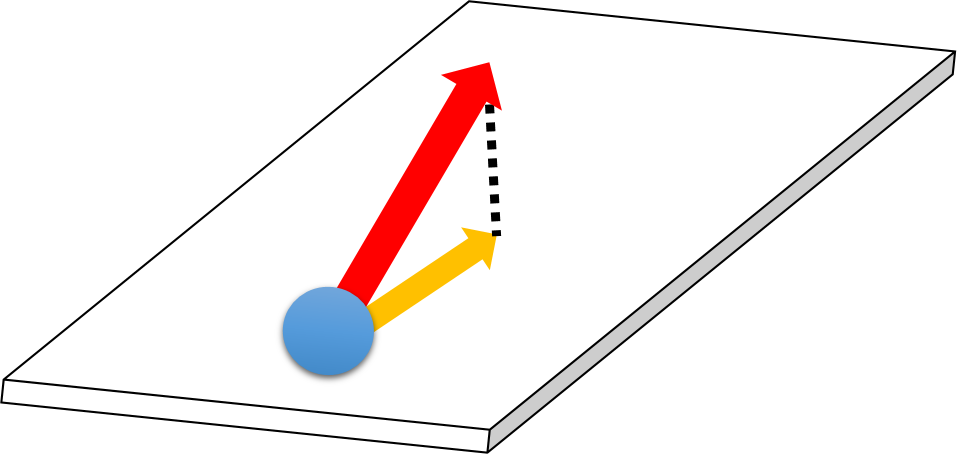
\includegraphics[width=0.35\linewidth]{png/repulsive.png}
		\caption[斥力の射影]{斥力の合計と決定した進行方向ベクトル}
		\label{fig:repulsive}
	\end{figure}
	
	\subsection{パラメータ設定}
	この章では,サイボーグインセクトを制御する場合のパラメータの設定について考える.
	\section{実験結果}
	\section{おわりに}
	\begin{thebibliography}{99}
		%%%%%%%%%%%%%%%%%%%%%
		% 参考文献リスト
		%%%%%%%%%%%%%%%%%%%%%
		\bibitem{}
	\end{thebibliography}
\end{document}